%%%%%%%%%%%%%%%%%%%%%%%%%%%%%%%%%%%%%%%%%
% Technical Abstract
%
%
%
%%%%%%%%%%%%%%%%%%%%%%%%%%%%%%%%%%%%%%%%%
%----------------------------------------------------------------------------------------
%       PACKAGES AND OTHER DOCUMENT CONFIGURATIONS
%----------------------------------------------------------------------------------------
\documentclass{article}
\usepackage[english]{babel} % English language/hyphenation
\usepackage[sfdefault,light,condensed]{roboto}
\usepackage[T1]{fontenc} % Use 8-bit encoding that has 256 glyphs
\usepackage{sansmath} % Math packages
\usepackage[ansinew]{inputenc}
\usepackage{graphicx} 
\usepackage{csquotes}
\linespread{2} % Line spacing - Palatino needs more space between lines
\usepackage[hmarginratio=1:1,top=32mm,columnsep=20pt]{geometry} % Document margins
\usepackage[colorlinks = true,
            linkcolor = blue,
            urlcolor  = blue,
            citecolor = blue,
            anchorcolor = blue]{hyperref} % For hyperlinks in the PDF
\usepackage{abstract} % Allows abstract customization
\renewcommand{\abstractnamefont}{\bfseries} % Set the "Abstract" text to bold
\renewcommand{\abstracttextfont}{\mdseries\itshape} % Set the abstract itself 
\usepackage{titlesec} % Allows customization of titles
\titleformat{\section}[block]{\large\scshape\centering}{\thesection.}{1em}{} % Change the look of the section titles
\titleformat{\subsection}[block]{\large}{\thesubsection.}{1em}{} % Change the look of the section titles
\newcommand{\horrule}[1]{\rule{\linewidth}{#1}} % Create horizontal rule command with 1 argument of height
\usepackage{fancyhdr} % Headers and footers
\pagestyle{fancy} % All pages have headers and footers
\fancyhead{} % Blank out the default header
\fancyfoot{} % Blank out the default footer
\fancyhead[C]{Aaron Brooks $\bullet$ 19 May 2015 $\bullet$ Molecular and Cellular Biology (MCB) Program} % Custom header text
\fancyfoot[C]{\thepage} % Custom footer text
\usepackage[backend=biber,
	style=nature,]{biblatex}% shortcuts
\addbibresource{refs.bib}
\usepackage[dvipsnames]{color}
\definecolor{light-gray}{gray}{0.85}
\usepackage[tikz]{bclogo}
\usepackage{framed}
\newenvironment{gbar}[1]{ %
\def\FrameCommand{{\color{#1}\vrule width 3 pt } \colorbox{light-gray}}%
\MakeFramed{\advance\hsize-\width\FrameRestore }}%
{\endMakeFramed}
\usepackage{setspace}

\newcommand{\tmsamp}[1]{\textsf{#1}}
\newcommand{\eg}{\emph{e.g.}}
\newcommand{\ie}{\emph{i.e.}}
\newcommand{\cm}{\tmsamp{cMonkey}}
\newcommand{\nwinf}{{\tmsamp{Inferelator}}}
\newcommand{\MEME}{{\tmsamp{MEME}}}
\newcommand{\halo}{{\emph{H. salinarum} sp. NRC-1 }}
\newcommand{\eco}{\emph{E. coli} K-12 MG1655 }
\newcommand{\tab}{{\hspace{5mm}}}
\newcommand{\rdb}{{\tmsamp{RegulonDB}}}
\newcommand{\simgt}{\,\hbox{\lower0.6ex\hbox{$\sim$}\llap{\raise0.6ex\hbox{$>$}}}\,}
\newcommand{\simlt}{\,\hbox{\lower0.6ex\hbox{$\sim$}\llap{\raise0.6ex\hbox{$<$}}}\,}
\newcommand{\egrine}{{\tmsamp{EGRIN 2.0}}}
\newcommand{\tmmathbf}[1]{\ensuremath{\boldsymbol{#1}}}
\newcommand{\tmop}[1]{\ensuremath{\operatorname{#1}}}

%----------------------------------------------------------------------------------------
%       TITLE SECTION
%----------------------------------------------------------------------------------------
\title{\vspace{-15mm}\fontsize{20pt}{10pt}\selectfont\textbf{Data-driven inference of dynamic transcriptional regulatory mechanisms in prokaryotes: a systems perspective}} % Article title
\author{
\large
{\textsc{ Aaron N. Brooks, PhD }}
%\normalsize \href{mailto:aaron.brooks@embl.de}{aaron.brooks@embl.de}\\[0.1mm] % Your email address
}
\date{}

%----------------------------------------------------------------------------------------
\begin{document}
\sansmath
\maketitle % Insert title
\thispagestyle{fancy} % All pages have headers and footers

\vspace{-5mm}\rule{\textwidth}{1pt}

\begin{abstract}
\noindent Microbes tailor their physiology to diverse environments despite having streamlined genomes and few regulators. Mechanisms by which microbes expand their genetic repertoire include modular reorganization of genetic expression through dynamic activity of complex gene regulatory networks (GRNs). Deciphering accurate GRNs is essential to understand how their topology contributes to cellular behavior. My dissertation developed computational methods to reverse engineer GRNs directly from genome sequence and transcriptome data. These data-driven models capture dynamic interplay of environment and genome-encoded regulatory programs for two phylogenetically distant prokaryotes: \textit{E. coli} (a bacterium) and \textit{H. salinarum} (an archaeon). The models reveal how distributions of \textit{cis}-acting gene regulatory elements (GREs) and the condition-specific influence of transcription factors (TFs) at each element produces environment-specific transcriptional responses. These regulatory programs partition and re-organize transcriptional regulation of genes within regulons and operons into modules that we call "condition-specific co-regulated modules", or \textit{corems}. Corems capture fitness-relevant co-regulation by different transcriptional control mechanisms acting across the entire genome. Organization of genes in corems defines a system-level principle for prokaryotic gene regulatory networks that extends existing paradigms of gene regulation and helps explain how microbes negotiate environmental change.
\end{abstract}

\section{Introduction}

Scientists have been trying to decode the contents of the genome even before the first report of the structure of DNA by Watson and Crick in 1953 \cite{watson_molecular_1953}. In 1986, efforts in this direction were greatly accelerated by the invention of automated DNA sequencing \cite{smith_fluorescence_1986}, which provided a technology capable of read genomes at a staggering rate \cite{check_hayden_technology:_2014}. Presently, investigators can use extensions of these technologies to address longstanding biological questions at an unprecedented scale, including: 


{
\setstretch{1.5}
\begin{itemize}
	\item How is DNA sequence transformed by the cell into molecular and cellular phenotypes?, and
	\item How does DNA sequence variation lead to altered phenotypes, including disease?
\end{itemize}
}

Despite many technical successes, however, these question remain largely unanswered. Outside of a few strictly Mendelian examples, the connection between genotype and phenotype is poorly understood. Phenotypes typically cannot be predicted from genotypes and, when they can, the variance explained by individual loci is low \cite{manolio_finding_2009}. This is especially true for human disease.  

The problem, it would seem, is not our ability to generate data; rather, it is our ability to interpret these data and use them for prediction. This is likely due to a complex, non-linear relationship between genetic information and physiology that we do not yet understand fully. What we do know is that complex phenotypes are somehow the result of how molecular machines read and interpret the genome in context of a dynamic, noisy chemical milieu.\\

\begin{bclogo}[logo =\bcoeil , barre = none , noborder = true]{Summary}%
\begin{gbar}{blue}
\setstretch{1.25}
{
The overarching goal of my work was to build quantitative models linking \textit{genetic architecture} to dynamic, condition-dependent \textit{transcriptional phenotypes} in microrganisms.
}
\end{gbar}
\end{bclogo}
\vspace{5mm}

\noindent I made progress towards this goal by developing genome-wide, data-driven models of transcriptional regulation in prokaryotes.  I decided to focus on transcriptional regulation because it is one of the first steps for extracting information from the genome.  The work was done in prokaryotes because they are tractable systems with relatively small genomes and a wide array of available genetic and molecular tools, allowing us to rapidly profile them in the lab and reducing computational requirements. I was able to demonstrate experimentally that these models are both highly-accurate and predictive. 

My original dissertation contained five primary sections: (1) a thorough review of prokaryotic gene regulatory mechanisms, with an emphasis on modularity in biological regulatory systems, (2) a description of existing approaches to reverse-engineer gene regulatory networks from high-throughput experimental data, (3) a detailed overview of the computational approaches developed, (4) a presentation of the successes (and limitations) of these new approaches, with an emphasis on how microbes leverage condition-specific TF-gene interactions to coordinate genomic expression, and, finally, (5) a discussion of the implications of these results for understanding the function and evolution of gene regulatory networks (GRNs).  

We\footnote{I will use the pronoun `we' to emphasize the collaborative nature of this research} were able to infer comprehensive and accurate GRNs directly from gene expression data for two microbes. We demonstrated how these networks refine our understanding of modular gene co-regulatory organization in prokaryotes. We introduce a new concept for genetic co-regulation, the co-regulated module or \textit{corem}. Organization of genes into corems better describes how functions, pathways, and regulatory mechanisms are organized to influence cellular fitness.

In this dissertation abstract, I will first provide a short background on gene regulation in prokaryotes. Thereafter, I will quickly summarize the methods we developed, highlight several key results, and briefly describe the significance and implications of our findings. 

\section{Why and how do microbes regulate their genomes?}

Microbes are complex adaptive systems that live in variable environments. The barrier separating a microbe from its environment is small, sometimes as little as a cell membrane. These unicellular organisms have evolved to embrace change from outside the cell, as well as from within (illustrated in Figure \ref{fig:chap1:cellsense}). Microbes deal with changes to their environment in several ways. 

Related to this work, microbes have evolved complicated regulatory systems that control expression of genes useful in different environments. A canonical example is the \textit{lac} operon in \textit{E. coli}. The \textit{lac} operon encodes several genes for lactose consumption. Lactose, however, is not always available and it is not the preferred carbon source for \textit{E. coli}. Since it would be energetically wasteful for the organism to produce these genes when lactose is unavailable or some preferred carbon source is available, the \textit{lac} operon has evolved to be expressed only in the presence of lactose as well as the absence of preferred carbon sources (like glucose). The ability to regulate expression of the genome is a function of regulatory proteins that control transcription. 

Gene expression is controlled at multiple production steps by several distinct molecular mechanisms. Generation of a protein product from a genetic locus can be regulated, for example, by controlling DNA structure and accessibility, transcription initiation, transcription elongation, or transcription termination. Bacterial mRNAs can even be regulated after transcription by small RNAs (sRNAs). My research focused specifically on the process of transcription initiation, which accounts for a large fraction of control for most genes. 

Proteins called transcription factors (TFs) regulate the initiation of transcription in response to environmental change (Figure \ref{fig:chap1:cellrelay}). These factors facilitate (activators) or prevent (inhibitors) recruitment of the RNA polymerase to gene start sites. TFs control specific genes by binding DNA sequences located in gene promoters. The sequence preference of a TF can be summarized by a motif logo. This logo is constructed by aligning all sites where a TF binds, counting the frequency of each nucleotide at each position and scaling by information content at each position (Figure \ref{fig:chap1:pssm}). In microbes, a majority of genomic regulatory sites that correspond to these motifs occur with 250 nucleotides of the transcription start site. We refer to these \textit{cis}-acting DNA sequences as gene regulatory elements or GREs. Importantly, most gene promoters contain GREs for multiple TFs. It is hypothesized that this feature of gene promoters produces a combinatorial "code" that leads to multiple, independent regulatory modes for each gene. 

\section{Regulation at a systems scale: gene regulatory networks (GRNs)}

One of the goals of systems biology is to determine what sequences a TF prefers to bind, as well as where and when it binds across the genome for every TF. This entails an array of regulatory interactions that can be cataloged, visualized, and analyzed as gene regulatory networks (GRNs). GRNs are a mathematical representation of interactions between genes and TFs. These networks are represented as a $n \times m$ matrix, where $n$ are genes, $m$ are TFs, and the value at $X_{n,m}$ can represent presence/absence of an interaction or more complex information about the association. Topological analysis of GRNs can reveal important features related to how cells process information \cite{barabasi_network_2004}. For example, it has been suggested that TF regulatory networks are hierarchical \cite{yu_genomic_2006}. In this model, a few "master" TFs propagate a regulatory cascade that ends in the activation or repression of many "lower-tier" TFs, which are responsible for the majority of transcriptional changes. An immediate prediction of this model is that global gene expression profiles will be more sensitive to removal of TFs at the top of the regulatory cascade compared to the bottom. These and other predictions leveraged from the topology of these networks can be tested directly through experimentation. 

Building comprehensive GRNs from experimental evidence, however, is intensive and expensive. While new technologies will provide faster and less costly alternatives, there is currently a demand to infer these networks directly from genome sequence and transcriptome data, which are less expensive to collect and widely available for a number of organisms. 

\section{\egrine: a system level model for the microbial regulatory genome} 

Towards the goal of developing methods to infer accurate GRNs from indirect gene expression measurements, we engineered a novel computational framework based on the \cm\ integrated biclustering algorithm originally described in \cite{reiss_integrated_2006}. \cm\ detects putatively modules of genes that tightly co-expression in a subset of the available gene expression measurements directly from the expresion data and genome sequence (Figure \ref{fig:bicluster}). These modules are constrained by sequence information (\textit{de novo} identification of conserved GREs in gene promoters), and functional association networks. The defining characteristic of \cm\ is that it combines all three types of data (expression, GREs and networks) together into an integrated model. It uses a stochastic optimization procedure to identify modules that best satisfy all three constraints, simultaneously.

We deployed \cm\ as an ensemble learning framework, ultimately modeling the condition-specific global transcriptional state of the cell as a function of combinations of transient TF-based control mechanisms acting at intergenic and intragenic promoters across the entire genome. For each model, we aggregated predicted co-regulatory associations across genes, GREs, and environments from many individual \cm\ models that were each trained on a subset of the available gene expression data. Ensemble methods have become increasingly popular in a number of contexts recently given their reported ability to reduce model variance and overfitting \cite{seni_ensemble_2010}. 

The final \egrine~ensemble or EGRIN 2.0 was constructed and mined using additional model aggregation and compilation procedures (Figure \ref{fig:egrin2:1}). These include, motif clustering \cite{van_dongen_using_2012} and scanning \cite{bailey_methods_1998}; gene co-regulation network construction and backbone extraction \cite{serrano_extracting_2009}; and network community detection \cite{ahn_link_2010}. These methods were used to identify GREs and their genome-wide locations, gene-gene co-regulatory associations, and corems, respectively.\\

\begin{bclogo}[logo =\bcinfo , barre = none , noborder = true]{EGRIN 2.0 enables:}%
\begin{gbar}{blue}
\setstretch{1.25}
{
(1) quantification of confidence in each regulatory association predicted by the model\\ (2) characterization of context-dependent regulatory mechanisms that occur infrequently in the data\\ (3) discovery of non-canonical regulatory mechanisms. 
}
\end{gbar}
\end{bclogo}
\vspace{5mm}

\noindent In the manuscript describing this model we provide evidence for each of these claims \cite{brooks_system_2014}. Here I briefly elaborate methods related to one of the more substantial biological findings from my work, the definition of condition-specific co-regulated modules (corems).

\section{Detection of condition-specific co-regulated modules (corems)}

Co-regulated modules or \textit{corems} are condition-specific modules discovered by EGRIN 2.0. Corems are significantly different from previous definitions of modular genetic regulation. In particular, corems encompass sets of genes that are potentially:

\begin{itemize}
	\item Regulated by multiple, independent TFs. 
	\item Contain subsets of operons and regulons, reflecting condition-specific generation of multiple transcriptional isoforms from an operon. 
	\item Include genes from multiple regulons and operons. 
	\item Range in size from small (3 genes) to large (100s of genes). 
	\item Vary in how often they are co-expressed, from rare ($<$1/10 of the observations) to common ($>$2/3 of the observations). 
\end{itemize}

\noindent An individual gene can belong to \textit{multiple} corems. These defining hallmarks of corems are illustrated in Figure \ref{fig:chap1:corem}.

Corems were discovered by post-processing the \egrine~ensemble as a weighted gene-gene co-regulatory association network with community detection algorithms. First, the ensemble of biclusters was transformed into a weighted gene-gene association graph $G$, where the nodes of $G$ are genes and the weight of edges between the nodes is proportional to their frequency of co-occurrence in biclusters:

\begin{equation}
w_{ij} = \frac{\left|B_i\cap B_j\right|}{\mathrm{min}(B_i,B_j)},
\end{equation}

\noindent where $w_{ij}$ is the weight of the edge between genes $i$ and $j$, $B_i$ is the set of all biclusters containing gene $i$. This gene-gene co-occurrence network represents how often \cm~ discovers co-regulation between every pair of genes in the genome.

After transforming the ensemble into a normalized graph, we removed edges that were statistically indistinguishable from noise by a multiscale backbone extraction procedure (with null hypothesis of uniform edge weight distribution given a node of degree $k$) \cite{serrano_extracting_2009}. Thus we retained all edges satisfying the following relation:

\begin{equation}
\alpha_{ij}=1-(k-1)\int_0^{w_{ij}}(1-x)^{k-2}dx\leq 0.05,
\end{equation}

\noindent where $\alpha_{ij}$ is the probability that the normalized weight $w_{ij}$ between genes $i$ and $j$ is compatible with the null hypothesis, and $k$ is the degree of gene $i$. For both inferred networks this procedure reduced the number of predicted gene-gene co-regulatory associations nearly 1,000 fold.

Following backbone extraction, we detected corems by applying a recently described link-community detection algorithm \cite{ahn_link_2010}. The algorithm computes a similarity score between all pairs of edges sharing a common keystone node, $k$, according to the Tanimoto coefficient, $T$:

\begin{equation}
T(e_{ik},e_{kj}) = \frac{a_i\cdot a_j}{|a_i|^2+|a_i|^2+a_i\cdot a_j},
\end{equation}

\noindent where

\begin{equation}
a_i=w_{ij}+\frac{\delta_{ij}}{k_i}\sum_{l\in n(i)}w_{il}.
\end{equation}

\noindent Here, $e_{ik}$ is the edge between gene $i$ and the keystone gene $k$, and $\delta_{ij}$ is the Kroenecker delta. The score reflects the similarity of gene neighborhoods adjacent to two edges sharing a gene, with the score increasing in value as the number and weight of overlapping adjacent edges increases. To transform the Tanimoto coefficient into a distance metric, we computed $1-T$.

Following scoring, the edges were aggregated by standard hierarchical clustering. The resulting tree is cut at many thresholds to optimize the local weighted density $D$ of the resulting clusters:

\begin{equation}
D=\frac{1}{M\langle w\rangle}\sum_{c\in C}m_c\langle w\rangle_c\left(\frac{m_c-(n_c-1)}{n_c(n_c-1)/2-(n_c-1)}\right),
\end{equation}

\noindent where $M$ is the total number of edges in the entire network, $\langle w\rangle$ is the average weight of edges in the entire network, $C$ is the set of all link communities at a given threshold, $m_c$ is the number of edges in community $c$, $\langle w\rangle_c$ is the average weight of edges in community $c$, and $n_c$ is the number of genes in community $c$. The density scoring metric $D$ had a clear optimum corresponding exactly to the cutoff that would have been chosen had we used an unweighted scoring metric. 

Since the communities produced by this algorithm are comprised of sets of edges, we defined a corem to include all genes incident to the edges in a community. Because of this definition, each gene can be a member of multiple  corems. In {\it H. salinarum}, this procedure generated 679 corems ranging in size from 3 to 377 genes, covering 1,363 of the 2,400 genes in the genome, and comprising 56,738 co-regulatory associations. In {\it E. coli}, we discovered 590 corems, ranging in size from 3 to 153 genes, covering 1,572 of 4,213 genes and 25,976 regulatory edges.

\section{Result: \egrine~discovers experimentally characterized regulatory mechanisms}

High quality GRNs need to be both comprehensive (high recall) and accurate (high precision). To evaluate the quality of \egrine, we compared its predictions on \eco to RegulonDB \cite{gama-castro_regulondb_2011}, an extensive, manually-curated, gold-standard of experimentally validated TF-gene interactions. \egrine~ accurately located binding sites for 60\% of experimentally characterized TFs in RegulonDB (53 out of 88 at FDR $\leq$ 0.05). At a standard precision cutoff of 25\%, \egrine~recovered 577 ``strong evidence'' TF-gene interactions, which is 2.7X as many validated interactions as algorithms that exclusively use expression data (Figure \ref{fig:egrin2:2:A}) \cite{faith_large-scale_2007,marbach_wisdom_2012}. As expected, the ensemble network had greater precision and recall than individual cMonkey runs. These results demonstrate that integrating complementary methods, such as \textit{de novo} GRE detection, improves the accuracy and coverage of inferred GRNs. 

\section{Result: Conditionally active GREs within operons generate multiple, overlapping, and differentially regulated transcript isoforms}

Some of the GREs discovered in \egrine~occur in non-canonical locations and lead to unexpected transcriptional behaviors, such as the subdivision of operons into multiple transcriptional units.  It was previously reported that the \halo transcriptome structure is modulated extensively by transcriptional elements located within operons and coding regions \cite{koide_prevalence_2009}. \egrine~recapitulated this phenomenon by sub-dividing operon genes into different corems. In all, the model predicted that nearly one-third of all \halo operons generate multiple transcript isoforms. Nearly half of these predictions of conditional operon structures were corroborated by experimentally mapped transcriptional breaks (hypergeometric pval = $4.2\times10^{-3}$; \cite{koide_prevalence_2009}). Often, these transcript boundaries were adjacent to GREs that coincide with experimentally determined TFB-binding sites (\cite{facciotti_general_2007}; Figure \ref{fig:egrin2:3:A}), reinforcing the accuracy of \egrine~predictions.

We further investigated whether \egrine~provides insight into downstream consequences of differentially regulating multiple transcript isoforms from the same operon. The \textit{dppAB1C2-oppD2-ykfD-VNG2342H} operon in \halo encodes an ATP-dependent dipeptide transporter. Some periplasmic binding proteins (like \textit{dppA}) have the reported ability to function in conjunction with different ABC transport systems, giving support to the hypothesis that \textit{dppA} can be regulated independently \cite{higgins_binding_1990}. Despite high co-expression of the entire operon in the training data (mean R$^{2}$ = 0.6 across 1495 conditions), \egrine~predicted that the genes of this operon are transcribed as three different isoforms, each co-regulated with genes of a different corem. These predicted isoforms were verified by experimentally mapped transcript boundaries (Figure \ref{fig:egrin2:3:A}). Each of these corems contains a different dpp isoform and is enriched for a different biological function, including vitamin biosynthesis, porphyrin metabolism, and purine biosynthesis, respectively (Figure \ref{fig:egrin2:3:B}). Predicted differential regulation of the core permease (\textit{dppB1C2-oppD2-ykfD-VNG2342H}) with porphyrin metabolism genes in the permease corem is consistent with the reported capability of this transporter system to uptake heme when it functions with a different solute binding protein (i.e., without \textit{dppA}; \cite{letoffe_housekeeping_2006}). Overall, \egrine~provided insight into the distinct environment-dependent functional associations of each transcript isoform.   

\section{Significance, Implications and Future Directions}

\egrine~explains how microbes tailor transcriptional responses to varied environments by modeling the genome-wide distribution of GREs, their organization within each promoter, and the consequences of their activities across the genome. The integrative model reveals regulatory mechanisms for reuse of genes in varying combinations, linking distinct molecular pathways. Corems represent a fundamental organizing principle of GRNs that captures fitness-relevant associations among genes, forging a link between the environment-dependent dynamics of transcriptional control and phenotype. 

%----------------------------------------------------------------------------------------
%       BIBLIOGRAPHY SECTION
%----------------------------------------------------------------------------------------

\newpage
%\bibliographystyle{abbrv}
%\bibliography{refs}
\printbibliography 

%----------------------------------------------------------------------------------------
%       FIGURES SECTION
%----------------------------------------------------------------------------------------
\newpage
\begin{figure}[h!]
    \centering
    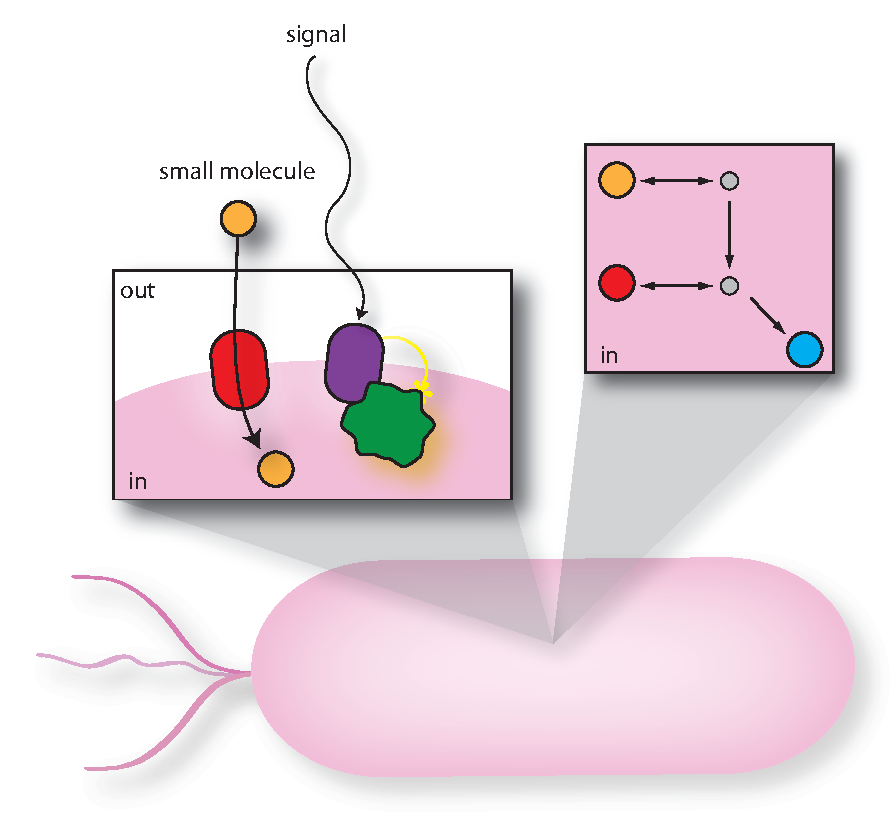
\includegraphics[width=0.6\textwidth]{figures/cell_env_signal_external}
    \caption[Microbes can sense internal and external changes to their environment]{Microbes can sense internal and external changes to their environment}
    \label{fig:chap1:cellsense}
\end{figure}

\begin{figure}[h!]
    \centering
    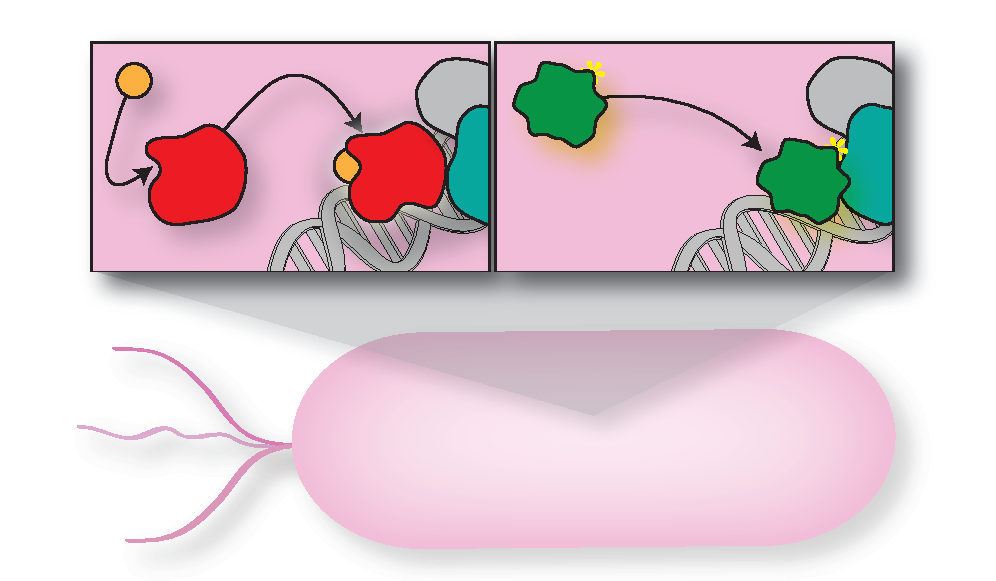
\includegraphics[width=0.6\textwidth]{figures/cell_env_internall}
 	\caption[Transcription factors (TFs) relay information about changes in the environment to regulate expression of the genome]{Transcription factors (TFs) relay information about changes in the environment to regulate expression of the genome}
    \label{fig:chap1:cellrelay}
\end{figure}

\begin{figure}[h!]
    \centering
    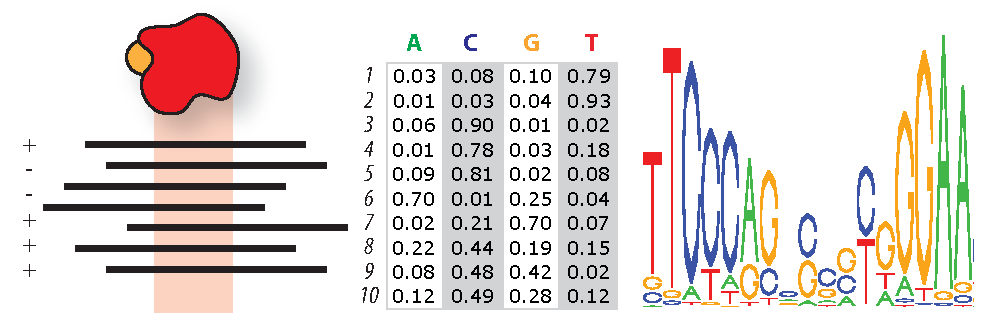
\includegraphics[width=0.9\textwidth]{figures/pssm}
 	\caption[Binding site alignment generates a position specific scoring matrix (PSSM) and motif logo that reflect the DNA sequence preference of a TF]{Binding site alignment generates a position specific scoring matrix (PSSM) and motif logo that reflect the DNA sequence preference of a TF}
    \label{fig:chap1:pssm}
\end{figure}

\begin{figure}[h!]
    \centering
    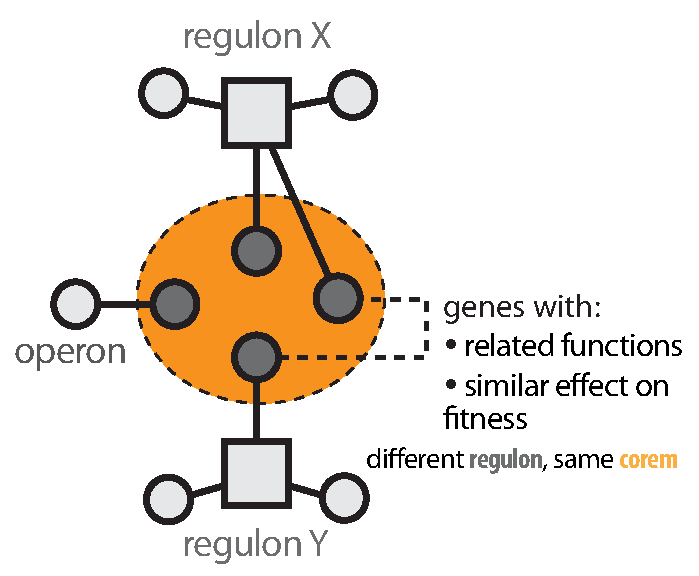
\includegraphics[width=0.6\textwidth]{figures/corem}
 	\caption[Corems are conditionally co-regulated sets of genes that can contain subsets of operons and regulons and be regulated by multiple transcription factors]{Corems are conditionally co-regulated sets of genes that can contain subsets of operons and regulons and be regulated by multiple transcription factors}
    \label{fig:chap1:corem}
\end{figure}

\begin{figure}[h!]
\centering
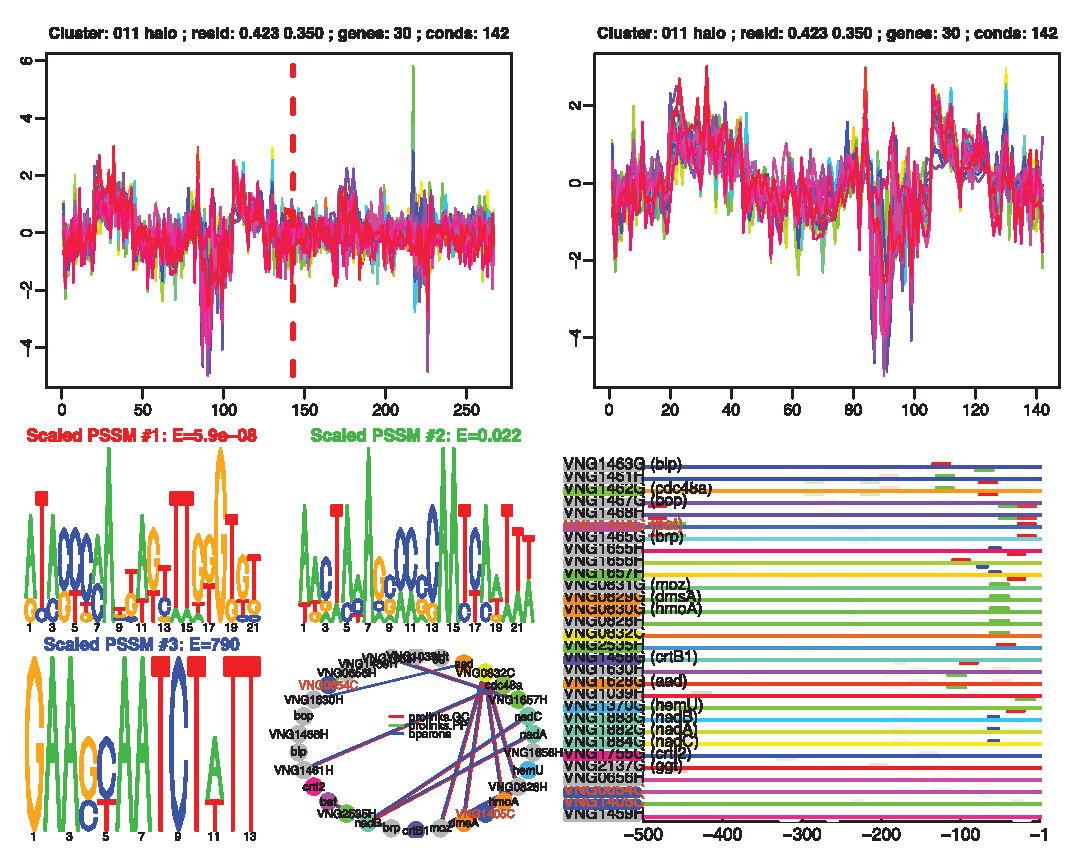
\includegraphics[width=0.9\linewidth]{figures/bicluster}
\caption[Bicluster: a conditionally co-regulated module identified by \cm\ containing genes with similar (1)  expression pattern, (2) upstream putative TF binding sequences (GREs), and (3) functions]{Bicluster: a conditionally co-regulated module identified by \cm\ containing genes with similar (1)  expression pattern, (2) upstream putative TF binding sequences (GREs), and (3) functions}
\label{fig:bicluster}
\end{figure}

\begin{figure}[h!]
    \centering
    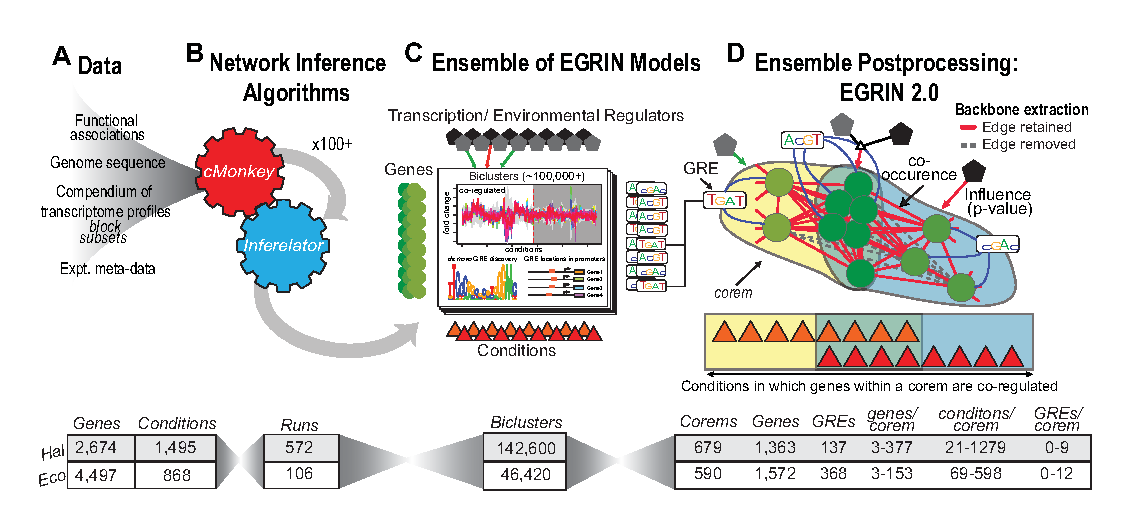
\includegraphics[width=0.9\textwidth]{figures/egrin2_fig1}
 	\caption[\egrine~model construction and summary statistics]{\egrine~model construction and summary statistics}
    \label{fig:egrin2:1}
\end{figure}

\begin{figure}[h!]
    \centering
    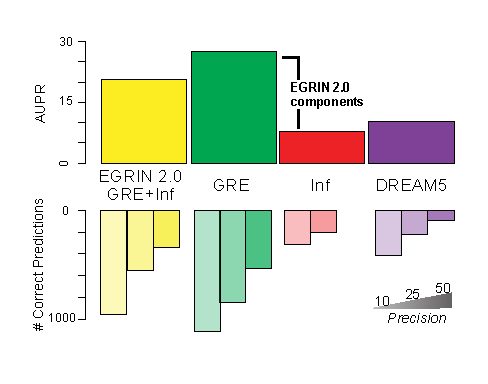
\includegraphics[width=0.75\textwidth]{figures/egrin2_AUPR}
 	\caption[\egrine~Model validation: performance on RegulonDB compared to other methods]{\egrine~Model validation: performance on RegulonDB compared to other methods}
    \label{fig:egrin2:2:A}
\end{figure}

\begin{figure}[h!]
    \centering
    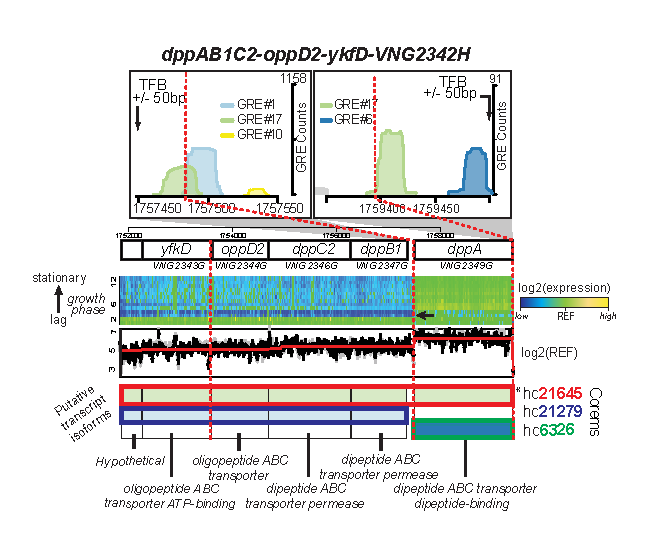
\includegraphics[width=0.8\textwidth]{figures/egrin2_dpp_1}
 	\caption[Transcriptional evidence for multiple transcript isoforms from the same operon, \halo ]{Transcriptional evidence for multiple transcript isoforms from the same operon, \halo }
    \label{fig:egrin2:3:A}
\end{figure}

\begin{figure}[h!]
    \centering
    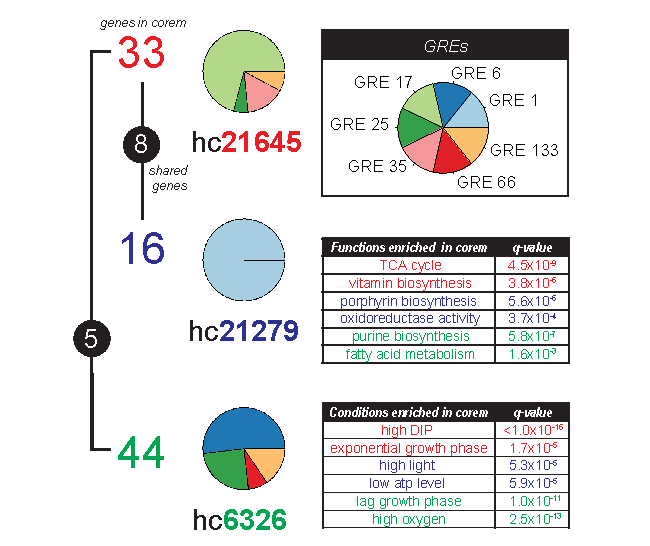
\includegraphics[width=0.65\textwidth]{figures/egrin2_dpp_2}
 	\caption[Functional consequences of multiple transcript isoforms from the same operon, \halo]{Functional consequences of multiple transcript isoforms from the same operon, \halo}
    \label{fig:egrin2:3:B}
\end{figure}


%----------------------------------------------------------------------------------------

\end{document}
